
\begin{frame}
	\frametitle{\textbf{2.5 : Lambda calcolo vs Lambda Expressions}}
	\begin{itemize}
		\item
			\textbf{Ricorsione}:\\\
			\begin{itemize}
				\item 
					Supponiamo di voler scrivere una lambda per calcolare il \textit{fattoriale} di un numero intero:\\\
					\begin{itemize}
						\item 
							In \textbf{Lambda Calcolo}, sarebbe:\\\ 
								\[
							 		let \quad Fact = \lambda n. if(n=0) \quad 1 \quad else \quad n*Fact(n-1)
								\]\\\				 
						\item 
							Che in \textbf{Java} sarebbe:
								\begin{figure}
									\centering
									
\includegraphics[width=0.5\linewidth]{image/factwrong.png}
									\label{fig:identity}
								\end{figure}
					\end{itemize}
				\item 
					Come sappiamo dal \textit{Lambda Calcolo}, questa espressione non è corretta, poiché la lambda, essendo \textit{funzione anonima}, non può sapere di chiamarsi \textit{Fact}.
			\end{itemize}
	\end{itemize}
\end{frame}

%----------------------------------------------------------------------------------------

\begin{frame}
	\frametitle{\textbf{2.5 : Lambda calcolo vs Lambda Expressions}}
	\begin{itemize}
		\item
			\textbf{Ricorsione - Continuo}:\\\
			\begin{itemize}
				\item 
					Possiamo quindi implementare un \textbf{Combinatore di Punto Fisso}.\\\
				\begin{itemize}
					\item
						Nel \textbf{Lambda Calcolo}, un noto \textit{Combinatore di Punto Fisso} è il seguente:\\\
							\[
								fix = \lambda f.(\lambda x.f(xxy))(\lambda x.f(\lambda y.xxy))
							\]
					\item
						In \textbf{Java} possiamo definire suddetto \textit{combinatore} come segue:\\\
							\begin{figure}
								\centering
								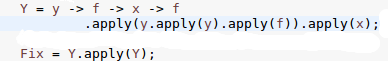
\includegraphics[width=0.8\linewidth]{image/fix.png}
								\label{fig:identity}
							\end{figure}
				\end{itemize}
			\end{itemize}
	\end{itemize}
\end{frame}

%----------------------------------------------------------------------------------------

\begin{frame}
	\frametitle{\textbf{2.5 : Lambda calcolo vs Lambda Expressions}}
	\begin{itemize}
		\item
			\textbf{Ricorsione - Continuo}:\\\
			\begin{itemize}
				\item 
					Applicando il \textit{Combinatore di Punto Fisso} al \textit{fattoriale}, otteniamo quindi:\\\
					\begin{itemize}
						\item 
							In \textbf{Lambda Calcolo}:\\\
								\[
									let \quad G = fix \quad Fact
								\]\\\
						\item 
							In \textbf{Java}:\\\
								\begin{figure}
									\centering
									
\includegraphics[width=0.8\linewidth]{image/factok.png}
									\label{fig:identity}
								\end{figure}
					\end{itemize}
			\end{itemize}
	\end{itemize}
\end{frame}